\documentclass{beamer}
\usepackage[utf8]{inputenc}
\usepackage{hyperref}

\title{Computação em Nuvem - Aula 5}
\subtitle{Fundamentação teórica\\
Prof. Me. Juliana Costa-Silva}

\usetheme{lucid}

\begin{document}
\frame{
 \titlepage
}

\frame{
    \frametitle{Roteiro de Aula}
    \tableofcontents
}
%-------------------------------------------------------
\section{Arquitetura Orientada a Serviços (SOA)}
\begin{frame}{Arquitetura Orientada a Serviços (SOA)}
Pensando em sistemas de amplo acesso, um fator relevante foi o desenvolvimento de Arquitetura Orientada a Serviços (SOA – \textbf{Service Oriented Architectures}) \cite{de2013cloud}.
\begin{itemize}
    \item Essa arquitetura consiste em decompor as funcionalidades de um sistema em serviços que podem ser reutilizados \cite{bernstein2014containers}.  
    \item O objetivo principal desse estilo arquitetural é promover a interoperabilidade entre aplicações.
    \item Neste caso, os serviços devem ser especificados de forma abstrata, sem dependências em relação a plataformas ou linguagens de programação.
\end{itemize}
\end{frame}
%--------------------------------------------
\begin{frame}{Web Services}

    $\rhd$ As requisições aos serviços em arquitetura SOA devem ser feitas por meio de tecnologias e padrões abertos. Neste contexto, foram introduzidos os Serviços Web (WS – \textit{Web Services}).\\
    \vspace{0.5cm}
    $\rhd$ Esses serviços \textbf{não são} aplicações Web para usuários finais. \\
    \vspace{0.5cm}
    $\rhd$ Eles são componentes de software cujas funcionalidades podem ser invocadas por outras aplicações por meio de requisições HTTP. \\
    \vspace{0.5cm}
    $\rhd$ Os dois modelos principais de Serviços Web são: \textcolor{red}{SOAP Web Services} e \textcolor{red}{RESTfull Web Services}.

\end{frame}
%--------------------------------------------
\subsection{Web Services SOA}
\begin{frame}{Tipos de Web Services}
\begin{exampleblock}{SOAP Web Services}
    \begin{itemize}
        \item  \textbf{*} Representou a primeira geração de serviços Web, em que as requisições aos serviços eram especificadas conforme o protocolo denominado SOAP (\textit{Simple Object Access Protocol}) e encapsuladas em mensagens HTTP.
        \item \textbf{*} As mensagens de requisição SOAP, a descrição dos serviços e a representação dos dados são todas baseadas em esquemas XML (\textit{Extensible Markup Language}).
    \end{itemize}
\end{exampleblock}
    
\end{frame}
%-------------------------------------------------------
\section{Web Services REST}
\begin{frame}{Tipos de Web Services}
    \begin{exampleblock}{REST (Representational State Transfer)}
        \begin{itemize}
            \item \textbf{*} É um estilo arquitetural para sistemas distribuídos;
            \item \textbf{*} Os serviços web que seguem os princípios e as restrições REST são então denominados RESTful Web Services.
        \end{itemize} 
    \end{exampleblock}
    \begin{exampleblock}{Restrições REST}
    \begin{itemize}
        \item \textbf{*} O sistema deve seguir o modelo cliente-servidor; não há manutenção de informações de estado por parte do servidor (stateless) \cite{tanembaum2007sd};
        \item \textbf{*} O sistema deve usar uma interface uniforme (padronizada) para acesso aos recursos disponíveis;
    \end{itemize}
        
    \end{exampleblock}
\end{frame}

\begin{frame}{Principais métodos HTTP usados em RESTful Web Services}
\begin{center}
   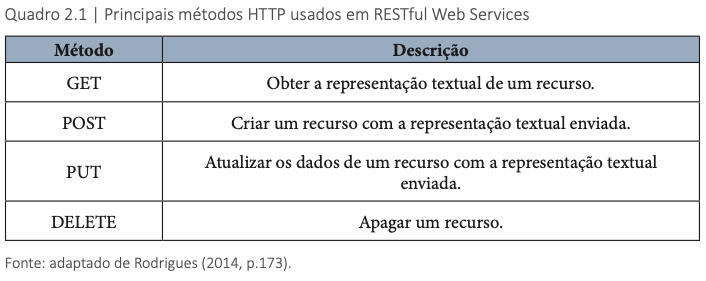
\includegraphics[width=0.95\linewidth]{fig/aula5/aula5_1.png}\\
   \tiny{\textbf{Fonte: } \cite{malheiros2019cc}.}
\end{center}
    
\end{frame}
%---------------------------------------------------------
\subsection{Recursos}
\begin{frame}{Recursos}
    \begin{exampleblock}{O que são recursos?}    	           \begin{itemize}
	    \item $\diamond$ O conceito de recurso é fundamental neste modelo de serviço web. 
	    \item $\diamond$ Um recurso é qualquer informação, acessível pelo serviço web, que pode ser endereçada através de um identificador padronizado (URI – \textit{Uniform Resource Identifier}) \cite{tanembaum2007sd}. 
	    \item $\diamond$ Os recursos devem ser representados em um formato textual, sendo o mais popular o JSON (\textit{JavaScript Object Notation}) \cite{nodejs2022api}. 
	    \item $\diamond$ Para manipulação dos recursos, são utilizados os métodos padronizados no protocolo HTTP. 
	\end{itemize}
    \end{exampleblock}
\end{frame}
%-------------------------------------------
\section{Atividade PARCIAL}
\begin{frame}{Atividade - PARCIAL}
    $\rhd$ Vamos testar a API RESTfull viacep;\\
    \vspace{0.5cm}
    $\rhd$ Acesse: \href{https://viacep.com.br/ws/01001000/json/}{https://viacep.com.br/ws/01001000/json/};\\
    \vspace{0.5cm}
    $\rhd$ Note que na url o termo 01001000é um CEP. Substitua esse termo por 86020080;\\
    \vspace{0.5cm}
    $\rhd$ Com suas palavras, explique a diferença entre um Web Service SOA e um Web Service RESTfull;\\
    \vspace{0.5cm}
    $\rhd$ De exemplos de sistemas que funcionam em Web Services SOA e RESTfull;\\
    \vspace{0.5cm}
    $\rhd$ Registre os links onde você fez a pesquisa para elaborar a sua resposta;
    
\end{frame}

%----------------------------------------
\begin{frame}{Referências}%[allowframebreaks]
 \tiny
 \begin{center}
 	\bibliographystyle{apalike}
	 \bibliography{ref}
 \end{center}
 \end{frame}

\end{document}